\documentclass[a4paper,12pt]{article}
\usepackage{amsmath}
\usepackage{amssymb}
\usepackage[polish]{babel}
\usepackage{polski}
\usepackage[utf8]{inputenc}
\usepackage{indentfirst}
\usepackage{geometry}
\usepackage{array}
\usepackage[pdftex]{color,graphicx}
\usepackage{subfigure}
\usepackage{afterpage}
\usepackage{setspace}
\usepackage{color}
\usepackage{wrapfig}
\usepackage{listings}
\usepackage{datetime}

\renewcommand{\onehalfspacing}{\setstretch{1.6}}

\geometry{tmargin=2.5cm,bmargin=2.5cm,lmargin=2.5cm,rmargin=2.5cm}
\setlength{\parindent}{1cm}
\setlength{\parskip}{0mm}

\newenvironment{lista}{
\begin{itemize}
  \setlength{\itemsep}{1pt}
  \setlength{\parskip}{0pt}
  \setlength{\parsep}{0pt}
}{\end{itemize}}

\newcommand{\linia}{\rule{\linewidth}{0.4mm}}

\definecolor{lbcolor}{rgb}{0.95,0.95,0.95}
\lstset{
    backgroundcolor=\color{lbcolor},
    tabsize=4,
  language=C++,
  captionpos=b,
  tabsize=3,
  frame=lines,
  numbers=left,
  numberstyle=\tiny,
  numbersep=5pt,
  breaklines=true,
  showstringspaces=false,
  basicstyle=\footnotesize,
  identifierstyle=\color{magenta},
  keywordstyle=\color[rgb]{0,0,1},
  commentstyle=\color[rgb]{0,0.5,0},
  stringstyle=\color{red}
  }

\begin{document}

\noindent
\begin{tabular}{|c|p{11cm}|c|} \hline
Grupa~4 & Katarzyna Kosiak i~Michał Folwarski & \ddmmyyyydate\today \tabularnewline
\hline
\end{tabular}

\section*{Zadanie~3 -- Rozmycie Gaussa w~CUDA}

Program rozmywa zadany obraz za pomocą algorytmu Gaussa z~maską o~wymiarach 5x5 korzystając z~technologii CUDA.

\noindent Zdefiniowano dwie metody używane w~CUDA:
\begin{lstlisting}
__device__ int getGauss(unsigned char* image,
                        int channel, int id,
                        int cols, int rows,
                        int arraySum)

__global__ void filter(unsigned char* inputImage,
                       unsigned char* outputImage,
                       int cols, int rows,
                       int arraySum)
\end{lstlisting}
Następnie zrównoleglono rozmywanie rzędów pikseli zadanego obrazu (po wcześniejszej alokacji pamięci zmiennych dla CUDA oraz zapisania w~nich obrazu wejściowego i~danych maski) zrealizowano w~sposób następujący:
\begin{lstlisting}
filter <<< grid, blockSize >>> (devInputImage,
                                devOutputImage,
                                inputImage.cols,
                                inputImage.rows,
                                arraySum);
//przepisanie obrazu wynikowego
cudaMemcpy(outputImage.ptr(),
           devOutputImage,
           imageMemSize,
           cudaMemcpyDeviceToHost);
\end{lstlisting}
Gdzie zmienna \verb!grid! to liczba bloków uruchomionych równolegle, a~zmienna \verb!blockSize! to liczba wątków w~każdym bloku. Funkcja \verb!filter! jedynie wywołuje trzykrotnie (dla każdego kanału) właściwą metodę rozmywającą obraz (getGauss).

Użyto jednowymiarowych bloków, ponieważ obraz zostaje przekazany do CUDA w~postaci jednowymiarowej tablicy, gdzie każde trzy kolejne elementy opisują jeden pikseel -- jego składowe (B,G,R).

Umieszczony poniżej wykres (Rysunek~1) pokazuje zależność czasu działania programu na maszynie z~kartą GeForce GTX 480  (maksymalny rozmiar bloku 1024, maksymalna liczba bloków 65535) od liczby wątków dla przykładowego obrazu o~rozmiarze boku około 1500px.

\begin{figure}[!hbtp]
 \centering
  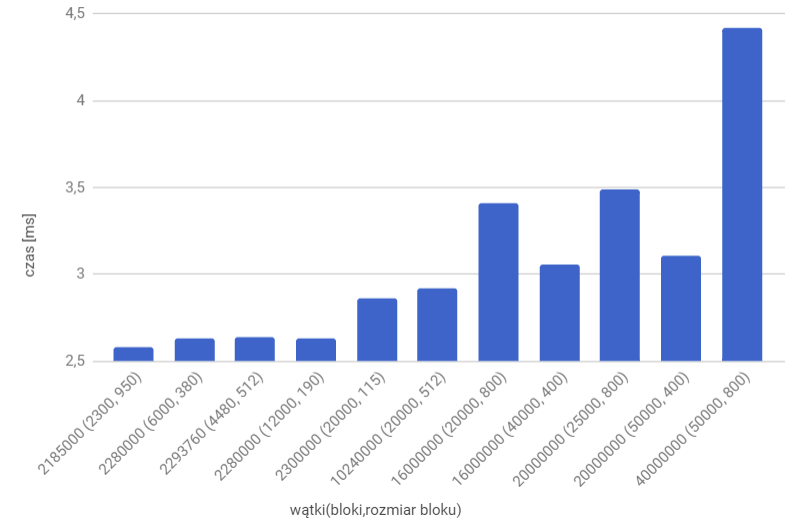
\includegraphics[width=0.9\textwidth]{wykres.png}
  \caption{Zależność czasu wykonania zadania od ilości wątków}
\end{figure}
Jak widać na wykresie, dla tego zadania nie ma większego znaczenia czy wykorzystuje się więcej bloków z~mniejszą ilością wątków czy mniej bloków z~większą ilością wątków (tak długo jak całkowita liczba wątków jest równa całkowitej liczbie pikseli, czyli nie wykonuje się zbędnych operacji typu tworzenie nieużytecznych wątków) -- wynika to z~faktu, że zadanie to nie wymaga dzielenia zasobów pomiędzy wątkami bloku.

Wykorzystanie wielu wątków w~bloku w~tym przypadku ma jedynie tę przewagę, że pozwala na przetwarzanie większych obrazów (bez przekroczenia limitu ilości bloków). Jedynie w~przypadku zbyt dużej liczby wątków w~stosunku do ilości pikseli widać, że lepsze czasy uzyskuje się przy użyciu mniejszej ilości wątków w~bloku a~większej ilości bloków -- wynika to z~architektury kart graficznych.

W~stosunku do niezrównoleglonego zadania na CPU uzyskano dla tego przypadku maksymalnie 700-krotne przyspieszenie. Liczba ta odbiega znacząco od przyspieszenia idealnego, wynika to m.in. z~faktu, że każdy z~wielu wątków musi zostać zainicjalizowany oraz że liczba wątków była wyznaczana empirycznie. GPU ma charakterystyczną architekturę i~wiele właściwości tej karty wpływa na osiągane przyspieszenie -- aby je poprawić, należałoby dokładnie zapoznać się z~użytym modelem karty graficznej.

\subsubsection*{Wnioski }
Zadanie udało się wykonać -- dokonano zrównoleglenia obliczeń. Wykorzystanie technologii CUDA spowodowało ogromne przyspieszenie procesu w~stosunku do tradycyjnego rozwiązania. Dzięki temu, że GPU posiada wiele jednostek mogących wykonać obliczenia, zrównoleglanie obliczeń jest bardzo skuteczne.

Zauważono jednak, że podczas projektowania rozwiązania każdego problemu trzeba wziąć pod uwagę ograniczenia wynikające z~architektury docelowej karty graficznej, a~skalibrowanie ilości wątków i~bloków wymaga niemałej wiedzy o~jej parametrach i~ich znaczeniu.
\end{document}
